\chapter{Introducción.}
En este capítulo primero de la memoria vamos a explicar las motivaciones que nos llevaron a pensar en realizar dicho proyecto, los objetivos que nos marcamos al principio cuando lo diseñamos, los materiales usados y la organización de esta memoria.

\section{¿Por qué decidimos hacer el proyecto?}
Al igual que muchos estudiantes de la Universidad de Málaga, yo suelo comer habitualmente en la cafetería de la facultad y hay mucha gente que se molesta cuando le piden que firme el papel con el que se lleva el recuento de los estudiantes que comen en las cafeterías para el descuento por ser estudiante. Además de dicho incoveniente hay un par de problemas más, que son lo molesto que es tener que firmar todos los días o habitualmente y las colas que se forman al tener que rellenar el nombre y la firma, por eso se decidió hacer una aplicación para terminales móviles con la que agilizar todo el proceso de firma y control de estudiantes, mediante la lectura de un código QR que tendría la información necesaria.

A medida que avanzaba el proyecto se vio que se podía ampliar no solo al comedor, si no también a alquiler de pistas o cualquier documento necesario en la Universidad de Málaga.

Además a mi me gusta la seguridad informática y vi en este proyecto una buena forma de aprender más sobre criptografía, particularmente la de clave pública, además vi una buena forma de aprender a programar para terminales android, debido al gran auge que tienen en este momento, y a crear aplicaciones web de las que no tenía ninguna idea. Al principio la aplicación web se penso en hacer directamente en java sin ninguna ayuda, pero se descartó ante la dificultad de encontrar un servicio de hosting gratuito, por lo que se decidió cambiar a una sugerencia que hizo director de proyecto de usar una plataforma que proporciona Google llamada Google App Engine, que es gratuito y se pueden crear aplicaciones web programadas con el lenguaje de programación Java y así tener la posibilidad de aprender otras apis, no solo Java2EE, para crear aplicaciones web en Google App Engine también hay que conocer aunque sea de forma básica Java2EE.

\section{Objetivos que queríamos conseguir.} 
El principal objetivo que queríamos conseguir era que la forma de firmar fuera muy fácil y que no fuera un mecanismo muy engorroso. Para ellos decidimos realizar una aplicación para smartphone android y una aplicación web para el almacenamiento y posterior comprobación de las firmas.

Por lo que empezamos a diseñar un sistema con el cual se puediera firmar digitalmente inicialmente solo un recibo y finalmente cualquier documento de la UMA agilizando dicho proceso.

%TODO: Hay poner algo de criptografía... xDDD

En la parte de la aplicación de android se decidió hacer una aplicación clara y que fuese fácil de usar. Para eso usamos la API nivel 14 que equivale a la versión 4.0 de android, llamada Ice Cream Sandwich. Se eligió porque proporciona una nueva forma de diseño de las interfaces, un nuevo tema  llamado Holo y proporciona muchas nuevas herramientas como por ejemplo son los ActionBar, que es una barra que permanece siempre en la parte superior de la pantalla en la que va acomodando a las necesidades en cada parte de la aplicación cambiando los botones según las necesidades, por ejemplo si estamos en la pantalla principal pues tendremos siempre visible el botón de añadir un nuevos recibo que abrirá el lector de códigos QR, se puede observar en la primera barra que se ve en la figura \ref{fig:actionBar}, sin embargo si estamos visualizando un recibo solo tendremos el botón de volver atrás, como se puede ver en la segunda barra de la figura \ref{fig:actionBar}, en la que se puede ver que al lado del icono de la aplicación una flechita que indica que es el botón para volver atrás.

\begin{figure}
  \centering
    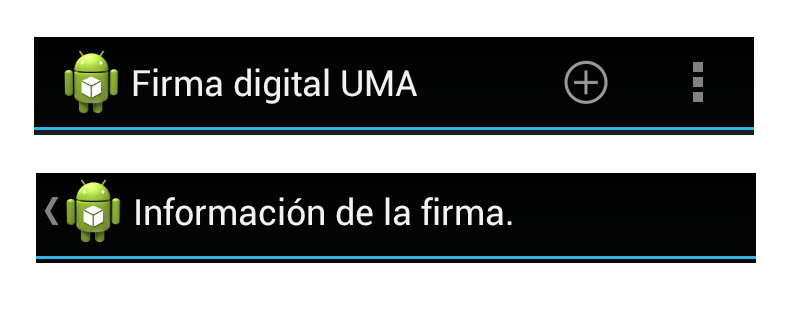
\includegraphics[scale=0.3]{./Introduccion/imagenes/actionbar.png}
  \caption{Action Bar.}
  \label{fig:actionBar}
\end{figure}

Al tomar la decición de programar para terminales con android 4.0 o mayor estuvimos sopesando los pros y los contras, y al final decidimos que la implantación de android 4.0 cada vez es mayor y que cada día hay más terminales con dicha versión, como se puede ver en este gráfico de la figura \ref{fig:graficoEvolucionAndroid} y podemos observar que a finales de agosto de este año la cantidad de usuarios afectados sería de más del 15\% de terminales como podemos ver en la figura \ref{fig:graficoUsoAndroid}, aunque todavía sigue reinando la versión 2.3.3, aunque creemos que el cambio a la versión 4.0 o superior será rápida debido a todas las ventajas que aporta y mucho más ahora que hace unos meses Google sacó una nueva versíon, la 4.1, llamada Jelly Bean y casi todas las compañías querrán actualizar sus terminales a la última versión, por lo que a pesar de dejar a un gran número de usuarios sin poder usar la aplicación preferimos usabilidad y elegancia frente a gran cantidad de usuarios, ya que estos llegarán a medida que sus compañias actualicen sus terminales.

\begin{figure}
  \centering
    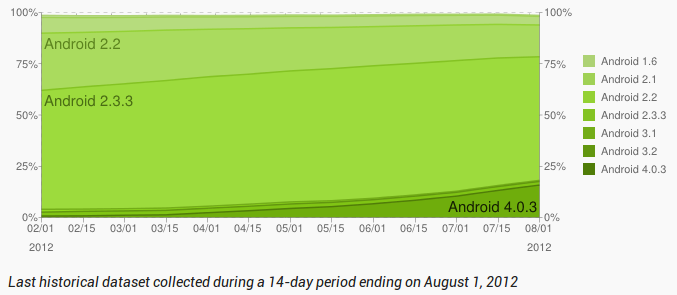
\includegraphics[scale=0.8]{./Introduccion/imagenes/graficoEvolucionAndroid.png}
  \caption{Gráfico de las versiones de android a finales de agosto del 2012.}
  \label{fig:graficoEvolucionAndroid}
\end{figure}

\begin{figure}
  \centering
    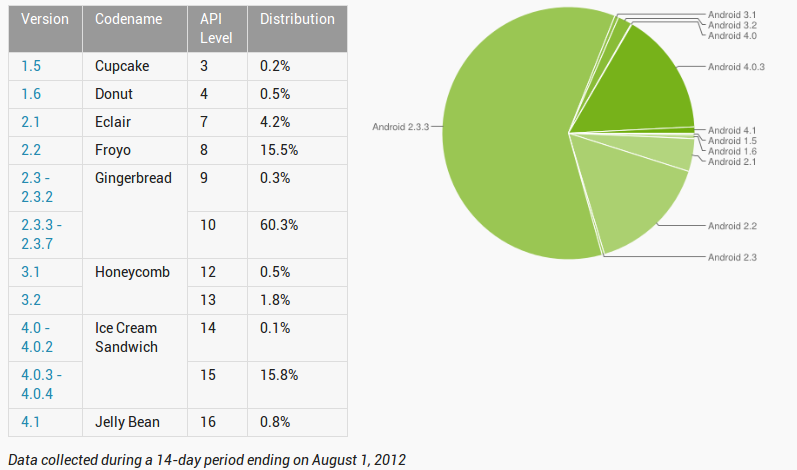
\includegraphics[scale=0.5]{./Introduccion/imagenes/graficoUsoAndroid.png}
  \caption{Gráfico del uso de las versiones de android a finales de agosto del 2012.}
  \label{fig:graficoUsoAndroid}
\end{figure}

En la parte del servidor al elegir la plataforma de Google, hubo muchas cosas que resultaron más fáciles a costa de tener que aprender a usar el SDK que ellos proporcionan, que como era una de las cosas por la que elegimos dicha plataforma no nos importó. Una de las cosas que nos facilitaba es la gestión de usuarios, que los gestiona google directamente al tener que loguearte en la aplicación web con una cuenta de Google Account. Toda la seguridad, mantenimiento, copias de seguridad, balanceos de carga y un largo etcetera también lo hacen ellos por lo que no habría que preocuparse de ello.

\section{Organización de la memoria.}
%TODO: rellenar al final...

\section{Material usado.}
Para la realización de este proyecto hemos usado un ordenador para todo lo que tiene que ver con la programación y un smartphone android para la depuración y prueba de la aplicación. 

El ordenador es un ordenador portatil normal, con Ubuntu 12.04 como sistema operativo, un procesador Pentium Dual Core a 2.2Ghz, 4 Gb de memoria ram.

El móvil es un Samsung Galaxy Nexus que fue el primer terminal en tener android 4.0 y meses después el primero en recibir android 4.1. Sus característica son una pantalla de 4.65 pulgadas Super Amoled con resolución de 1280 x 720, procesador dual-core a 1.2Ghz, HSPA+, NFC, Wifi, GPS, etc.

\begin{figure}
  \centering
    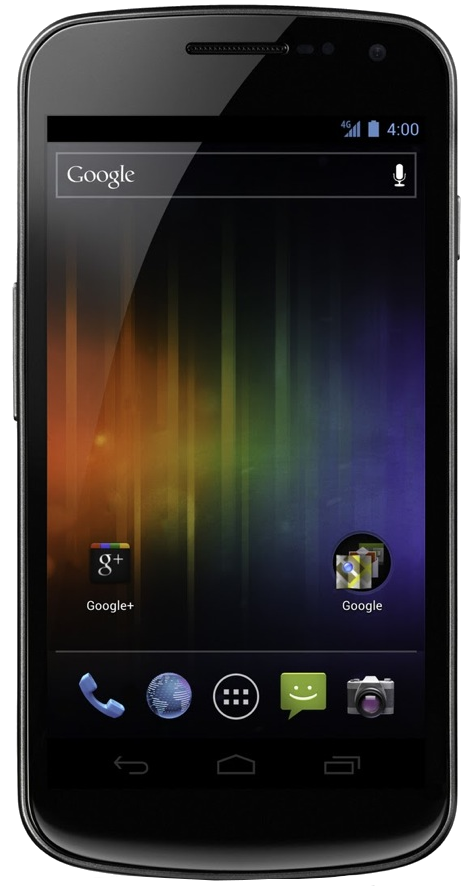
\includegraphics[scale=0.3]{./Introduccion/imagenes/nexus.png}
  \caption{Samsung Galaxy Nexus.}
  \label{fig:nexus}
\end{figure}
